\documentclass{neu_handout}
\usepackage{url}
\usepackage{amssymb}
\usepackage{amsmath}
\usepackage{marvosym}
\usepackage{graphicx}
\usepackage[pdftex]{graphicx}
\usepackage{subfigure}
\graphicspath{ {images/} }
\everymath{\displaystyle}

% Professor/Course information
\title{Homework 1 - Part 2}
\author{Emily Dutile}
\date{January 2018}
\course{CS7295}{Info Viz}

\begin{document}


\section*{Visualization 1}

\subsection*{1. Lie Factor}

Taking the largest peak and comparing it with the smallest (measurable) peak, we get the following:\\

Lie Factor = $ \frac{(2.2 - 1.2)}{1.2} * 100 = 83.33 $
\\

Lie Factor = $ \frac{(29035 - 16024)}{16024} * 100 = 81.2 $
\\

Lie Factor = $ \frac{83.33}{81.2} = 1.03 $
\\

There is a very small, to what I would consider, no lie factor here with the 2D data (altitude and mountain) represented by a 2D image. The scale on the left is in increments of 5,000 ft, while the scale on the right is in meters. Since the lines of the scale don't perfectly line up, the scales do accurately represent the data. For example, 8,000 m is roughly 26,246 ft. As we can see, the 8,000 m line is slightly above 25,000 ft. Due to this, our lie factor is  very slightly over 1 isn't over or understanding the data in the visual.


\subsection*{2. Design Critique}

The Se7en Summits creatively and accurately represents the seven summits of the tallest mountains on each continent. This visualization is similar to a bar chart. Here, we have two attributes encoded: a line mark with the vertical spacial position channel for the elevation in feet/meters and the horizontal spatial position channel is for the mountain. These two channels are representing our quantitative and categorical attribute respectively. The data, which is the altitude of mountains illustrated through the use of triangles (shape) and area (size), are line markers. In order to identify each mountain, the author creatively  uses different mountain images which all have somewhat unique characteristics and colors for the channel. Over all, this visual is very creative, accurate, and a bit difficult to critique. One change I would make visually is to make the background a bit darker in comparison to the white text, frame, and grid lines. The use of the text boxes above the mountain makes it easy to identify the mountain, location, and it's elevation. The second visual below the chart representing the prominence rank in the world is easy to under stand and it doesn't get lost in the bold images. If it weren't a requirement, I would remove one scale and keep it to either feet or meters The conversion of feet to meters would be kept in the textbox. We could also consider reordering the mountains in ranking order in order to not have a ranking centered under the Great Pyramid of Giza.


\subsection*{3. Re-design}

Please see appendices for redesign.



\section*{Visualization 2}

\subsection*{1. Lie Factor}

Looking at the peak of the Atlantic Cod and the lowest point, we calculate the following lie factor:\\

Lie Factor = $ \frac{(3.0-0.5)}{0.5} * 100 = 500 $
\\

Lie Factor = $ \frac{(3500000 - 750000)}{750000} * 100 = 366.67 $
\\

Lie Factor = $ \frac{500}{366.67} = 1.36 $
\\

\subsection*{2. Design Critique}

In general, adding additional dimensions (volume) to the data just adds clutter and confusion most visualizations, and this is a good unjustified 3D example. It makes it harder to quickly and accurately analyze the data when 3D is not needed. To improve this visualization, I would keep the marks as lines but change it to a line plot to show the decreasing number of specific fish in the sea in the time series and also keeping the horizontal and vertical position. This could be done with different line colors to represent as the author looked to do. I would remove the colorful table of the fish counts all together or at least remove the color. The shading seems like it should be associated with the plot, but it doesn't - it is only the fish color on the left hand side. These line plots could be represented as one graph, or 5 graphs with the same scale. I think the most effective way would be a stacked bar chart in order to show the total fish population count, and then showing the different fish categories by the given color. The table could be kept to give more granular information. By removing the 3D chart which is more difficult due to the perspective distortion and occlusion, this visualization can become cleaner and more effective.


\subsection*{3. Re-design}

Please see appendices for redesign.



\newpage

\appendix
\section{Appendices}

\begin{figure}[h]
\centering
{
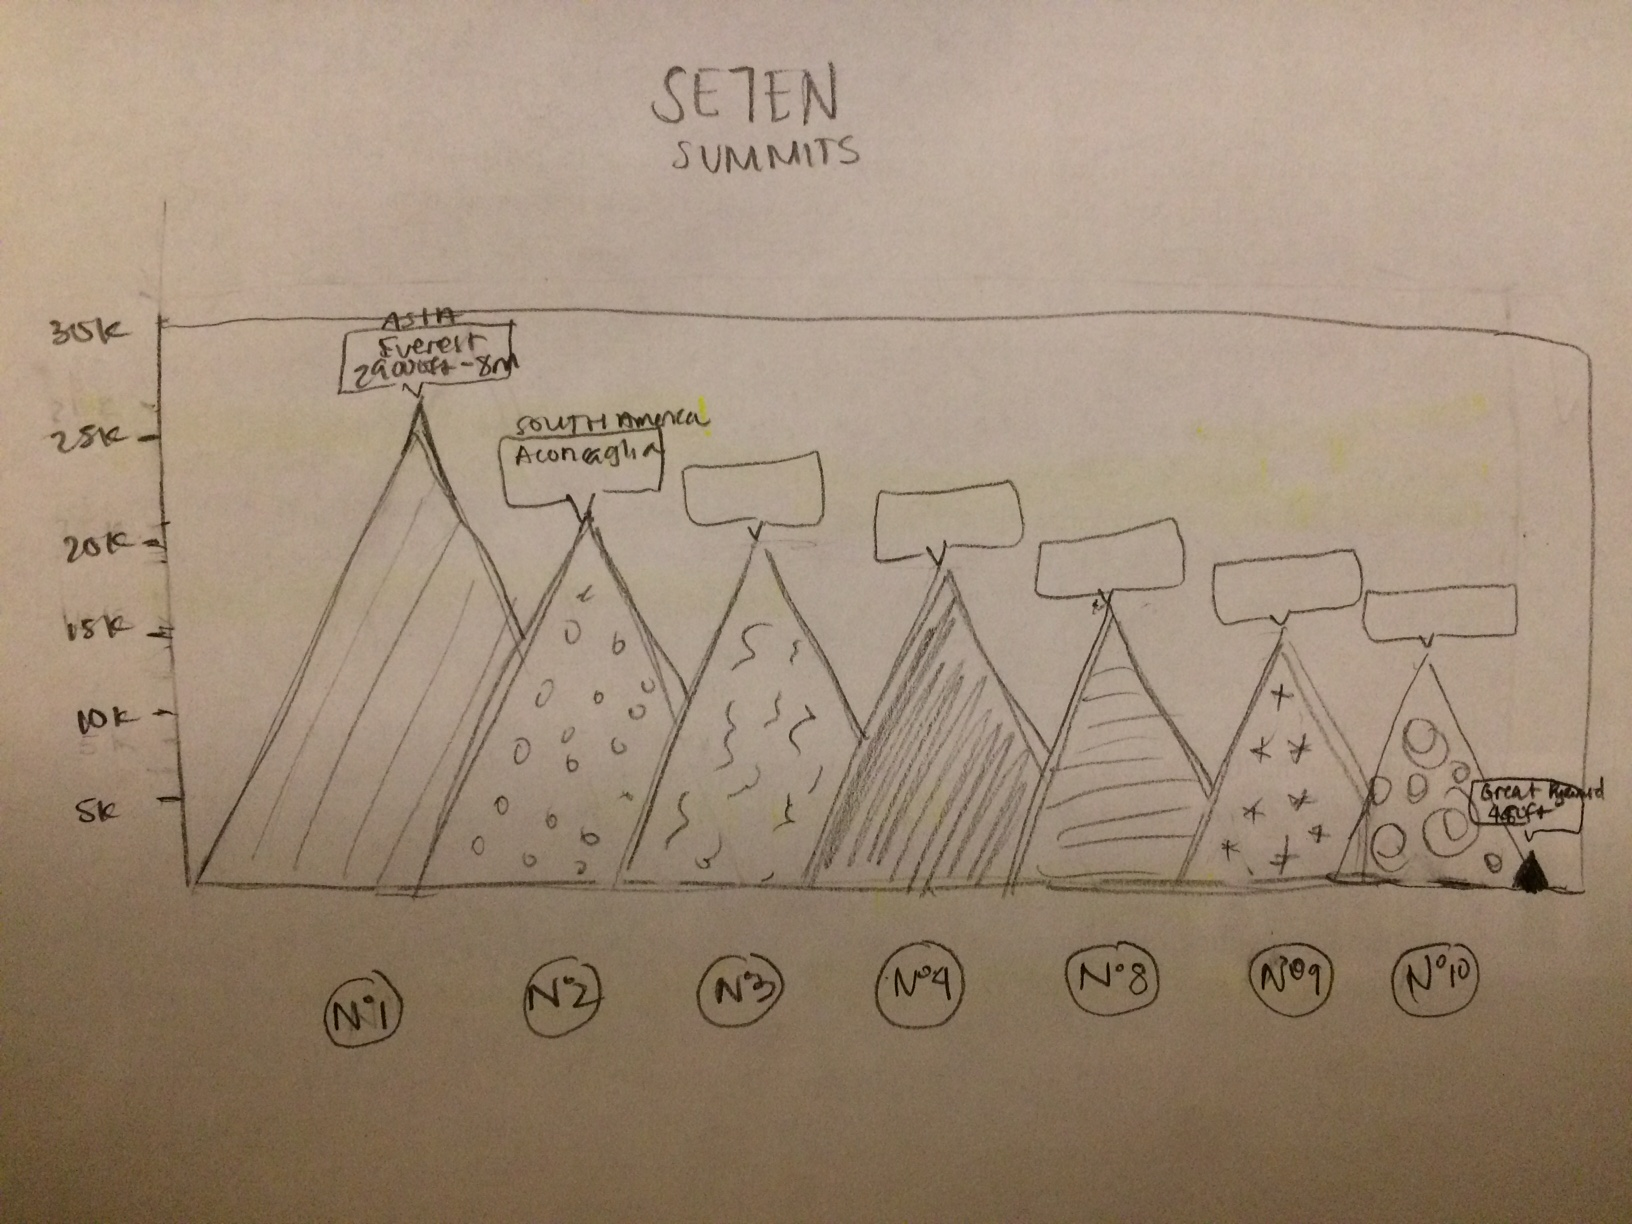
\includegraphics[width=0.5\linewidth]{part2_1}
}
\end{figure}


\begin{figure}[h]
\centering
{
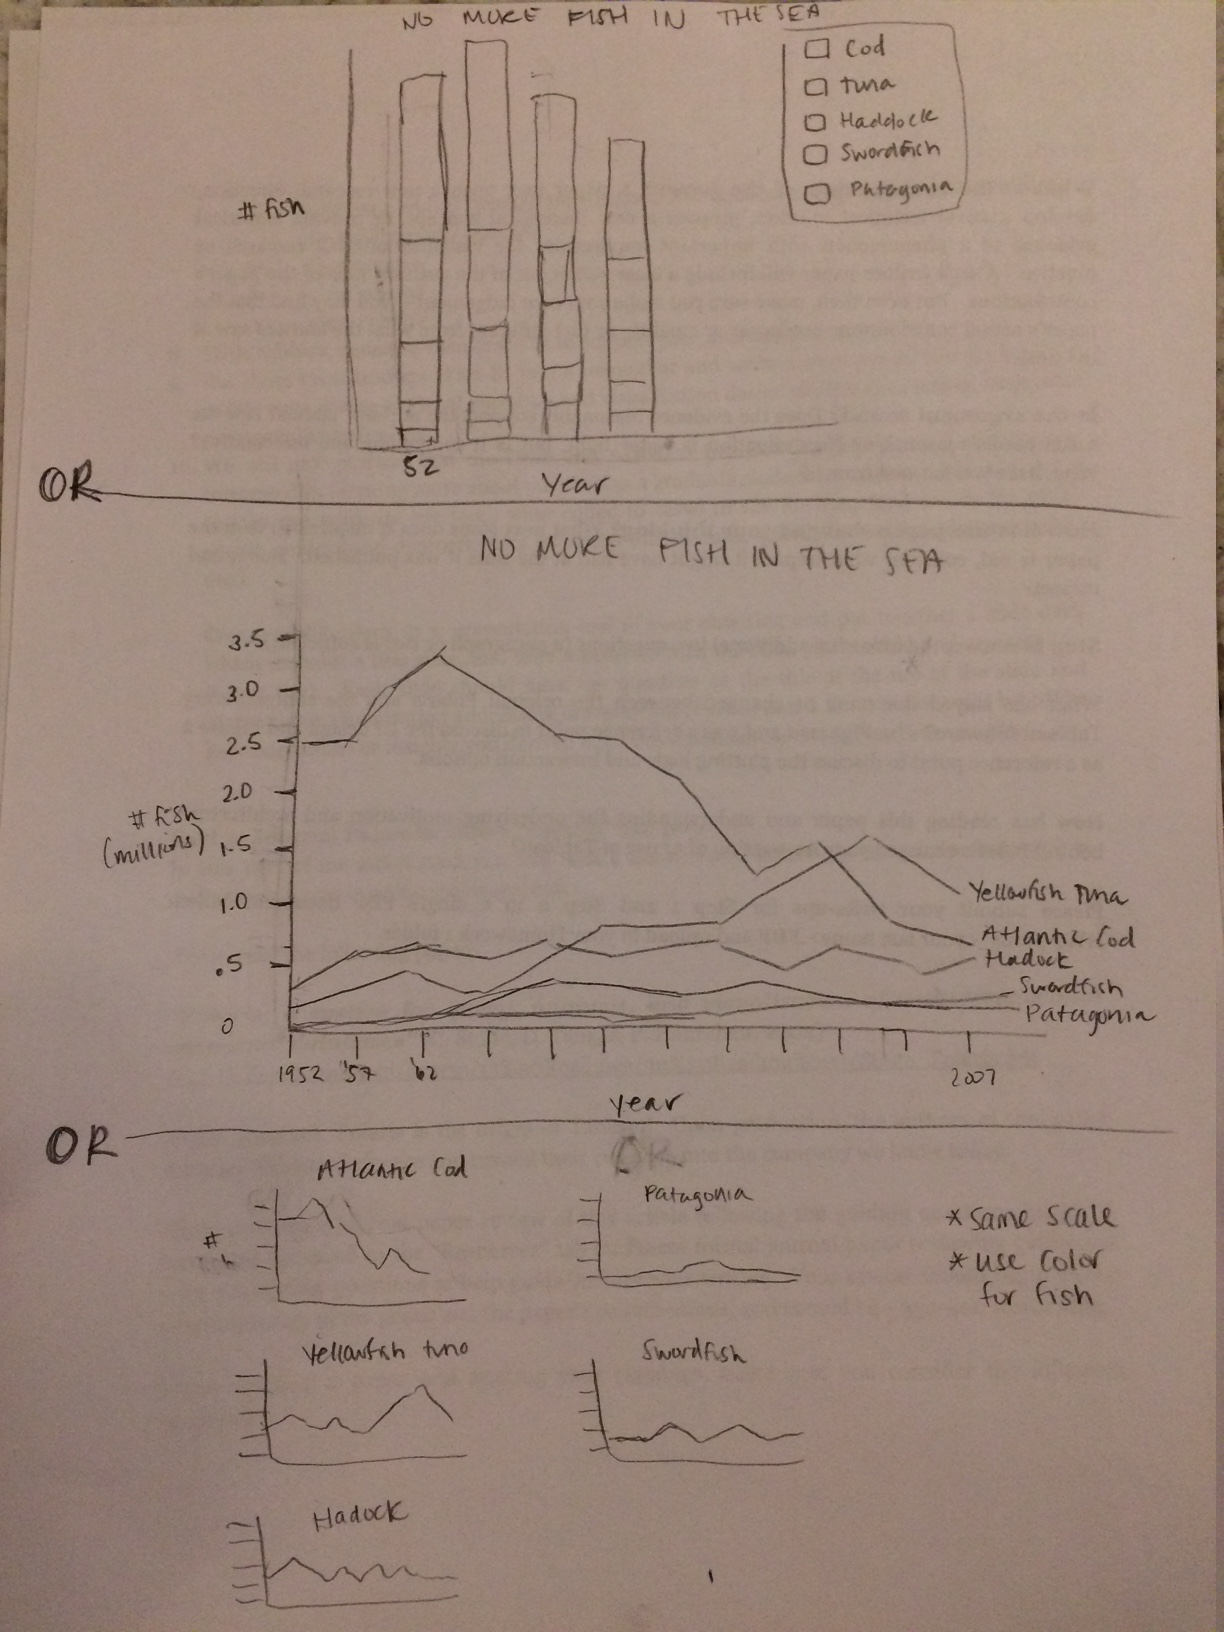
\includegraphics[width=0.4\linewidth]{part2_2}
}
\end{figure}


\end{document}
